% 2010 年湖北卷理科第 18 题：四面体 ABOC，P 为 AC 中点，O 为被遮挡的顶点。
% 来源 PDF：普通高考/2010/2010湖北理.pdf，SHA-256 2cfb3d100d55f89c58fe4475caf29f039496afbd0f16d7a7d07857eed5759f55。
% 原页：第 2 页（A3 三栏）第 1 栏，书页码 598。
% 重绘依据：按 600 dpi 原页，可见面 ABC 用实线（CA、CB、AB），被遮挡的三条棱
%   CO、OB、AO 用虚线；P 点在 AC 上并标出实心点。O 在投影图中位于 A、B 连线的上方。
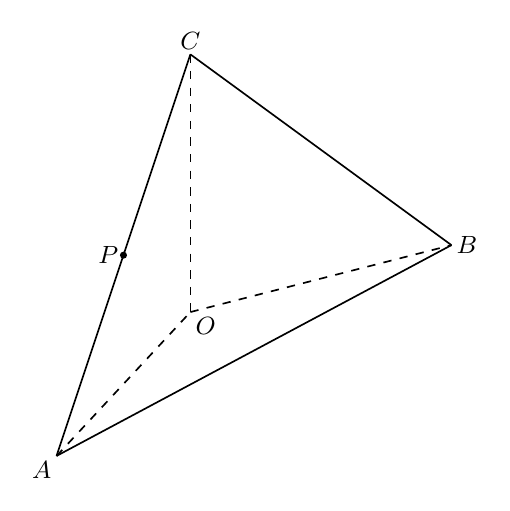
\begin{tikzpicture}[scale=0.85, semithick, every node/.style={inner sep=1.6pt, font=\small}]
  \coordinate (A) at (0,0);
  \coordinate (B) at (5.9,3.15);
  \coordinate (C) at (2.0,6.0);
  \coordinate (O) at (2.0,2.15);
  \coordinate (P) at (1.0,3.0);
  % 可见棱
  \draw (A) -- (B);
  \draw (A) -- (C);
  \draw (B) -- (C);
  % 被遮挡的棱
  \draw[dashed] (C) -- (O);
  \draw[dashed] (O) -- (B);
  \draw[dashed] (A) -- (O);
  % 中点 P
  \fill (P) circle (1.5pt);
  % 标注
  \node[below left]  at (A) {$A$};
  \node[right]       at (B) {$B$};
  \node[above]       at (C) {$C$};
  \node[below right] at (O) {$O$};
  \node[left]        at (P) {$P$};
\end{tikzpicture}
